
% Table is required for multicolumn package with beamer
\documentclass[table]{beamer}

\usepackage{pucv_jz}

\title{Análisis de Datos}
\subtitle{Estadística Computacional}
\author[J.Z.O-2023]{Juan Zamora Osorioo\\\url{juan.zamora@pucv.cl}}
\institute[PUCV]{Instituto de Estadística\\Pontificia Universidad Cat\'olica de Valpara\'iso}
%\date{\today}


\begin{document}

\begin{frame}[plain]
    \titlepage
\end{frame}

%\begin{frame}
%\frametitle{Contents}
%\tableofcontents
%\end{frame}

% \section{Motivation}

%\begin{frame}
%\frametitle{Contents}
%\tableofcontents[currentsection]
%\end{frame}


\begin{frame}
    \frametitle{Terminología}
    \begin{block}{Dato}
        \begin{itemize}
            \item Del latín \emph{datum}, es una representación simbólica, un atributo o una característica de una entidad o cosa.
            \item \emph{Observación} de un fenómeno con una escala de medida.
        \end{itemize}
    \end{block}
    \begin{block}{Población objetivo (universo de estudio) ($\Omega$)}
        \begin{itemize}
            \item Colección de todas las unidades posibles consideradas.
        \end{itemize}
    \end{block}
    \begin{block}{Muestra}
        \begin{itemize}
            \item Lo que conocemos de una población.
            \item Es una imagen (sinopsis) del todo.
            \item $M = \bparens{\omega_{1} , \omega_{2} , \ldots , \omega_{n}} \subseteq \Omega$ muestra de $n$ datos.
        \end{itemize}
    \end{block}
\end{frame}

\begin{frame}
    \frametitle{Terminología}
    \begin{block}{Dato}
        \begin{itemize}
            \item Del latín \emph{datum}, es una representación simbólica, un atributo o una característica de una entidad o cosa.
            \item \emph{Observación} de un fenómeno con una escala de medida.
        \end{itemize}
    \end{block}
    \begin{alertblock}{Cuidado}
        \begin{itemize}
            \item Recordar que el dato no corresponde a la realidad misma, sino a su representación
        \end{itemize}
    \end{alertblock}
\end{frame}

\iffalse
\begin{frame}
    \frametitle{Terminología -- Tipos de datos}
    \begin{block}{Según escala de medida}
        \begin{itemize}
            \item Categóricos: escala nominal.
            \item Ordinales: escala ordinal.
            \item Contínuos: escala intervalar o de razón.
        \end{itemize}
    \end{block}
\end{frame}
\fi

\begin{frame}
    \frametitle{Datos categóricos / discretos / nominales / cualitativos}
    \begin{exampleblock}{Ejemplos}
        \begin{itemize}
            \item Género: masculino, femenino, no binari@.
            \item Nacionalidad: Chile, Argentina, Perú, etc.
            \item Color de ojos.
            \item Ha salido fuera del país: sí, no.
        \end{itemize}
    \end{exampleblock}
    \begin{center}
        \includegraphics[height=0.5\textheight]{Map_of_South_America}
    \end{center}
\end{frame}

\begin{frame}
    \frametitle{Datos ordinales}
    \begin{exampleblock}{Ejemplos}
        \begin{itemize}
            \item Edad: 0, 1 año, 2 años, etc.
            \item Cantidad de hijo/as: 0, 1, 2, 3, etc.
            \item Talla de zapatos.
            \item Niveles de educación (?).
        \end{itemize}
    \end{exampleblock}
    \begin{center}
        \includegraphics[height=0.5\textheight]{estrellitas}
    \end{center}
\end{frame}

\begin{frame}
    \frametitle{Datos continuos}
    \begin{exampleblock}{Ejemplos}
        \begin{itemize}
            \item Tiempo que demora en caer un objeto.
            \item Distancia al lanzar una piedra.
            \item Precio de una acción en la bolsa.
            \item Temperatura.
            \item Ángulo que apunta una ruleta.
            \item Segundos desde 1970 (?).
        \end{itemize}
    \end{exampleblock}
    \begin{center}
        \includegraphics[height=0.4\textheight]{ruleta}
    \end{center}
\end{frame}

\begin{frame}
    \frametitle{Escalas de medida}
    \begin{center}
        \small
        \begin{tabular}{c|m{0.15\textwidth}|m{0.35\textwidth}|m{0.22\textwidth}}
            \hline
            Escala & Operaciones empíricas básicas & Estructura matemática de grupo & Estadísticos invariantes \\
            \hline
            \hline
            \textbf{Nominal} & Igualdad & Grupo de permutaciones $x' = f \parens{x}$, con $f \parens{x}$ cualquier sustitución uno a uno & Número de casos, moda, correlación de contingencia \\
            \hline
            \textbf{Ordinal} & Mayor o menor & Grupo isotónico $x' = f \parens{x}$, con $f \parens{x}$ cualquier función monótona & Mediana, percentiles (cuantiles) \\
            \hline
            \textbf{Intervalar} & Igualdad de intervalos o diferencias & Grupo lineal general $x' = a x + b$ & Media, desviación estándar, correlaciones \\
            \hline
            \textbf{De razón} & Igualdad de razones & Grupo de similaridad $x' = a x'$ & Coeficiente de variación \\
            \hline
        \end{tabular}
        % \includegraphics[width=0.95\textwidth]{tipos_datos}
    \end{center}
\end{frame}

\begin{frame}
    \frametitle{Terminología -- Tipos de datos}
    \begin{block}{Según cantidad de variables}
        \begin{itemize}
            \item Univariados.
            \item Bivariados.
            \item Multivariados.
        \end{itemize}
    \end{block}
    \begin{alertblock}{Cuidado}
        Muchos fenómenos se representan por medio de datos mezclados (estructurados o no estructurados).
    \end{alertblock}
\end{frame}

\begin{frame}
    \frametitle{Conjunto de datos}
    \begin{block}{Qué es}
        \begin{itemize}
            \item Recordar: una representación de la cosa.
            \item Descripciones de distintas instancias de un mismo fenómeno.
            \item Similar a una ``muestra''.
            \item Representados como tuplas, matrices, tensores, grafos, imágenes, etc.
        \end{itemize}
    \end{block}
    \begin{equation*}
        \begin{blockarray}{*{5}c}
            \text{Dato} & \text{Atributo } 1 & \text{Atributo } 2 & \cdots & \text{Atributo } p \\
            \begin{block}{(*{5}{c})}
                1 & x_{1 , 1} & x_{1, 2} & \cdots & x_{1 , p} \\
                2 & x_{2 , 1} & x_{2, 2} & \cdots & x_{2 , p} \\
                \vdots & \vdots & \vdots & \ddots & \vdots \\
                n & x_{n , 1} & x_{n, 2} & \cdots & x_{n , p} \\
            \end{block}
        \end{blockarray}_{n \times p}
    \end{equation*}
    %\includegraphics[width=0.9\textwidth]{dataset_abstracto}
\end{frame}

\begin{frame}
    \frametitle{Conjunto de datos como matriz}
        % \includegraphics[width=0.9\textwidth]{dataset_pizza}
    \begin{exampleblock}{Ejemplo: despachos de una cadena de pizzerías}
        \begin{equation*}
            \begin{blockarray}{*{5}c}
                \text{Entrega} & \text{Tiempo entrega} & \text{Temperatura} & \cdots & \text{Sucursal} \\
                \begin{block}{(*{5}{c})}
                    1 & 35.1 & 68.3 & \cdots & \text{Este } \parens{1} \\
                    2 & 25.2 & 71.0 & \cdots & \text{Este } \parens{1} \\
                    \vdots & \vdots & \vdots & \ddots & \vdots \\
                    1266 & 35.7 & 60.8 & \cdots & \text{Oeste } \parens{2} \\
                \end{block}
            \end{blockarray}
        \end{equation*}
    \end{exampleblock}
    \begin{block}{Decisiones / transformaciones}
        \begin{itemize}
            \item ¿Unidades?
            \item ¿Cómo representar datos categóricos?
            \item 1, 2, 3, 4.
            \item 0001, 0010, 0100, 1000.
        \end{itemize}
    \end{block}
\end{frame}

\begin{frame}
    \frametitle{Frecuencias}
    \begin{exampleblock}{Ejemplo: alumnos presentes}
        \begin{itemize}
            \item S, N, S, N, S, S, S, N, S, S.
        \end{itemize}
    \end{exampleblock}
    \begin{block}{Frecuencias}
        \begin{itemize}
            \item Absoluta:
                \begin{itemize}
                    \item $n_{S} = 7$.
                    \item $n_{N} = 3$.
                \end{itemize}
            \item Relativa:
                \begin{itemize}
                    \item $f_{S} = \frac{n_{S}}{n} = \frac{7}{10} = 0.7$.
                    \item $f_{N} = \frac{n_{N}}{n} = \frac{3}{10} = 0.3$.
                \end{itemize}
        \end{itemize}
    \end{block}
\end{frame}

\begin{frame}
    \frametitle{¿Y los datos continuos?}
    \begin{block}{Agrupando}
        \begin{itemize}
            \item Podemos agrupar por intervalos.
        \end{itemize}
    \end{block}
    \begin{exampleblock}{Ejemplo: notas de control}
        \begin{itemize}
            \item 28, 35, 42, 90, 70, 56, 75, 66, 30, 89, 75, 64, 81, 69, 55, 83, 72, 68, 73, 16.
        \end{itemize}
        \begin{center}
            \begin{tabular}{c|c|c|c|c}
                0 -- 20 & 21 -- 40 & 41 -- 60 & 61 -- 80 & 81 -- 100 \\
                \hline
                $n_{1} = 1$ & $n_{2} = 3$ & $n_{3} = 3$ & $n_{4} = 9$ & $n_{5} = 4$ \\
                \hline
                $f_{1} = \frac{1}{20}$ & $f_{2} = \frac{3}{20}$ & $f_{3} = \frac{3}{20}$ & $f_{4} = \frac{9}{20}$ & $f_{5} = \frac{4}{20}$ \\
            \end{tabular}
        \end{center}
    \end{exampleblock}
\end{frame}

\iffalse
\begin{frame}
    \frametitle{Transformaciones}
    \begin{block}{Cambio de unidades}
        \begin{itemize}
            \item Transformación debe ser ``invertible''.
        \end{itemize}
    \end{block}
    \begin{center}
        \includegraphics[width=0.9\textwidth]{agrupados}
    \end{center}
\end{frame}
\fi

\begin{frame}
    \frametitle{Visualización: gráfico de torta}
    \begin{center}
        \begin{tikzpicture}
            \pie[text=pin, hide number]{2/Nada de satisfecho, 8/No satisfecho, 40/Satisfecho, 40/Muy satisfecho, 10/Perfectamente satisfecho}
        \end{tikzpicture}
        %\includegraphics[width=0.48\textwidth]{pie}
    \end{center}
\end{frame}

\begin{frame}
    \frametitle{Visualización: gráfico de torta}
    \begin{center}
        \includegraphics[width=0.48\textwidth]{torta_meganoticias}
        %\includegraphics[width=0.48\textwidth]{torta_fixmega}
        \begin{tikzpicture}
            \pie[rotate=90, radius=1.9]{13/Aprueba, 4/{No sabe, no responde}, 5/No aprueba ni desaprueba, 78/Desaprueba}
        \end{tikzpicture}
    \end{center}
\end{frame}

\begin{frame}
    \frametitle{Visualización: gráfico de barras}
    \begin{exampleblock}{Ejemplo: alumnos presentes}
        \begin{itemize}
            \item S, N, S, N, S, S, S, N, S, S.
        \end{itemize}
    \end{exampleblock}
    \begin{center}
        \includegraphics[width=0.49\textwidth]{bar1}
        \includegraphics[width=0.49\textwidth]{bar2}
    \end{center}
\end{frame}

\begin{frame}
    \frametitle{Visualización: gráfico de barras apilado}
    \begin{block}{Frecuencia absoluta versus relativa}
        \begin{itemize}
            \item ¿Cuál es la diferencia entre utilizar la frecuencia absoluta y la relativa?
        \end{itemize}
    \end{block}
    \begin{center}
        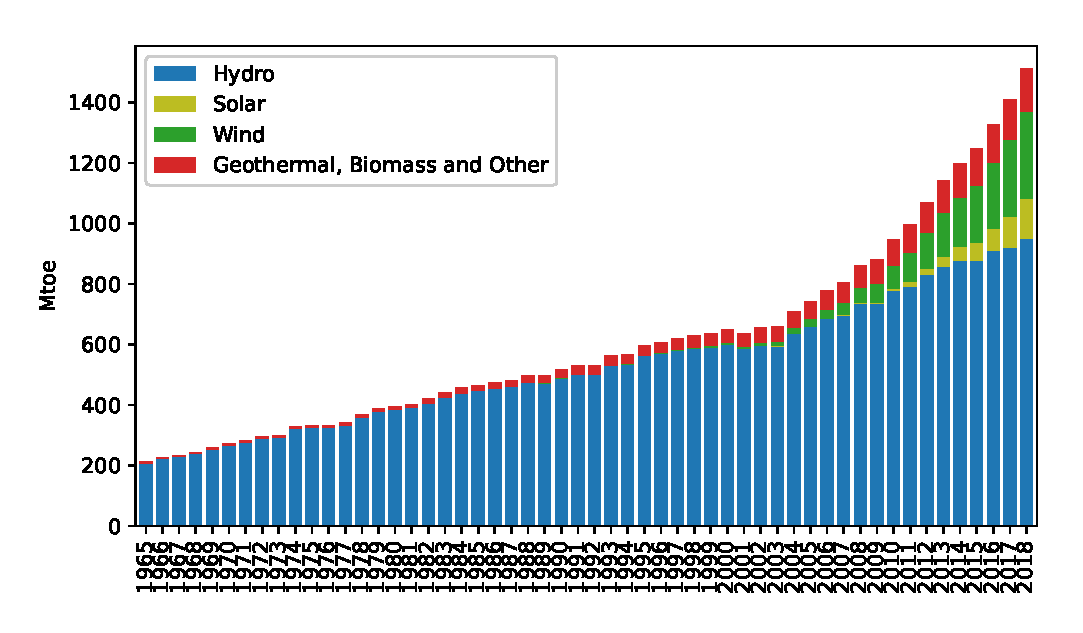
\includegraphics[width=0.49\textwidth]{energy_consumption_renewable_sources}
        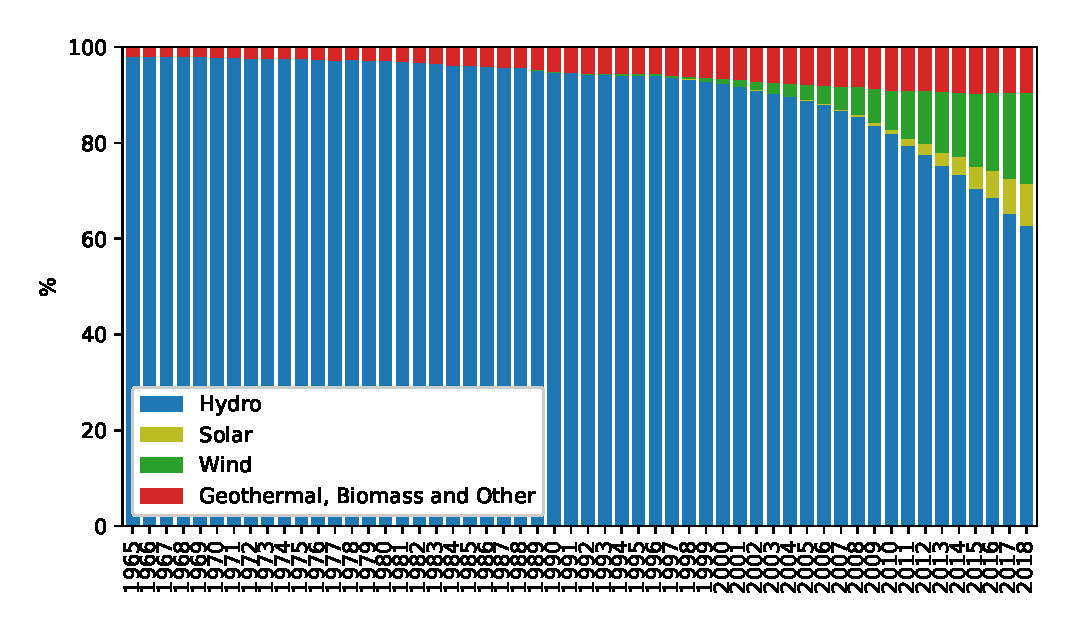
\includegraphics[width=0.49\textwidth]{energy_consumption_renewable_sources_percentage}
    \end{center}
\end{frame}

\begin{frame}
    \frametitle{Visualización: gráfico de barras}
    \begin{center}
        \includegraphics[width=0.49\textwidth]{barras_noticias}
        \includegraphics[width=0.49\textwidth]{barras_errorchile}
    \end{center}
\end{frame}

\begin{frame}
    \frametitle{Visualización: gráfico de barras}
    Porcentaje que se paga de impuestos:
    \begin{center}
        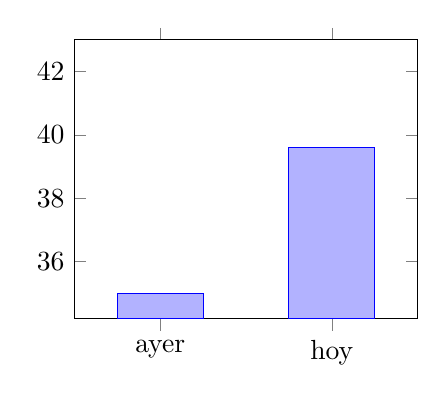
\begin{tikzpicture}
            \begin{axis}[
                ybar,
                bar width=0.5,
                xticklabels={ayer,hoy},
                xtick=data,
                width=0.49\textwidth,
                ymax=43,
                xmin=-0.5,
                xmax=1.5,
                no markers,
                ]
                \addplot+ coordinates {(0, 35) (1, 39.6)};
            \end{axis}
        \end{tikzpicture}
        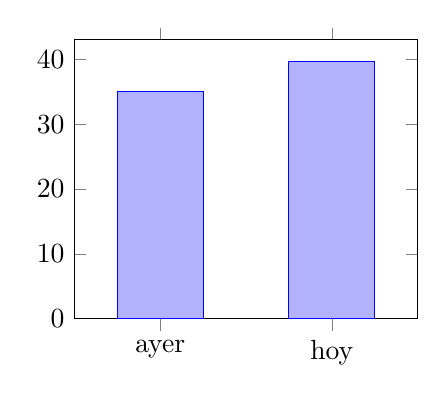
\begin{tikzpicture}
            \begin{axis}[
                ybar,
                bar width=0.5,
                xticklabels={ayer,hoy},
                xtick=data,
                width=0.49\textwidth,
                ymin=0,
                ymax=43,
                xmin=-0.5,
                xmax=1.5,
                no markers,
                ]
                \addplot+ coordinates {(0, 35) (1,39.6)};
            \end{axis}
        \end{tikzpicture}
        %\includegraphics[width=0.8\textwidth]{barras_ejemplomalo}
    \end{center}
\end{frame}

\begin{frame}
    \frametitle{Gráfico de tallo-hojas}
    \begin{block}{Notas de control}
        \begin{itemize}
            \item 28, 35, 42, 90, 70, 56, 75, 66, 30, 89, 75, 64, 81, 69, 55, 83, 72, 68, 73, 16.
        \end{itemize}
    \end{block}
    \begin{center}
        \begin{tabular}{c|l}
            0 & \\
            1 & 6 \\
            2 & 8 \\
            3 & 05 \\
            4 & 2 \\
            5 & 56 \\
            6 & 4689 \\
            7 & 02355 \\
            8 & 139 \\
            9 & 0 \\
        \end{tabular}
    \end{center}
\end{frame}

\begin{frame}
    \frametitle{Gráfico de tallo-hojas}
    \begin{block}{Notas de control}
        \begin{itemize}
            \item 28, 35, 42, 90, 70, 56, 75, 66, 30, 89, 75, 64, 81, 69, 55, 83, 72, 68, 73, 16.
        \end{itemize}
    \end{block}
    \begin{center}
        \includegraphics[width=0.49\textwidth]{stem_histo1}
    \end{center}
\end{frame}

\begin{frame}
    \frametitle{Gráfico de tallo-hojas}
    \begin{block}{Notas de control}
        \begin{itemize}
            \item 28, 35, 42, 90, 70, 56, 75, 66, 30, 89, 75, 64, 81, 69, 55, 83, 72, 68, 73, 16.
        \end{itemize}
    \end{block}
    \begin{center}
        \includegraphics[width=0.49\textwidth]{stem_histo1}
    \end{center}
    \begin{alertblock}{Heurística: ley de Benford}
        Dependiendo del dominio, tienden a agruparse en los números más pequeños, especialmente dominios abiertos de razón.
    \end{alertblock}
\end{frame}

\begin{frame}
    \frametitle{Histograma}
    \begin{block}{Notas de control}
        \begin{itemize}
            \item 28, 35, 42, 90, 70, 56, 75, 66, 30, 89, 75, 64, 81, 69, 55, 83, 72, 68, 73, 16.
        \end{itemize}
    \end{block}
    \begin{center}
        \includegraphics[width=0.49\textwidth]{stem_histo1}
        \includegraphics[width=0.49\textwidth]{stem_histo2}
    \end{center}
\end{frame}

\iffalse
\begin{frame}
    \frametitle{Gráfico de tallo-hoja: ¿qué esperamos?}
    \begin{block}{Número desconocido}
        \begin{itemize}
            \item ¿Con qué dígito comienza?
        \end{itemize}
    \end{block}
\end{frame}

\begin{frame}
    \frametitle{Gráfico de tallo-hoja: ¿qué esperamos?}
    \begin{block}{Número desconocido}
        \begin{itemize}
            \item ¿Con qué dígito comienza?
        \end{itemize}
    \end{block}
    \begin{center}
        \includegraphics[angle=270, width=0.9\textwidth]{primer_digito}
    \end{center}
\end{frame}
\fi

\begin{frame}
    \frametitle{Histograma -- continuo}
    \begin{center}
        \includegraphics[width=\textwidth]{histo_diferentesanchos}
    \end{center}
\end{frame}

\begin{frame}
    \frametitle{Histograma -- ejemplos demanda eléctrica}
    \begin{center}
        \begin{tabular}{ccc}
            Pan de Azúcar & Quillota & San Joaquín \\
            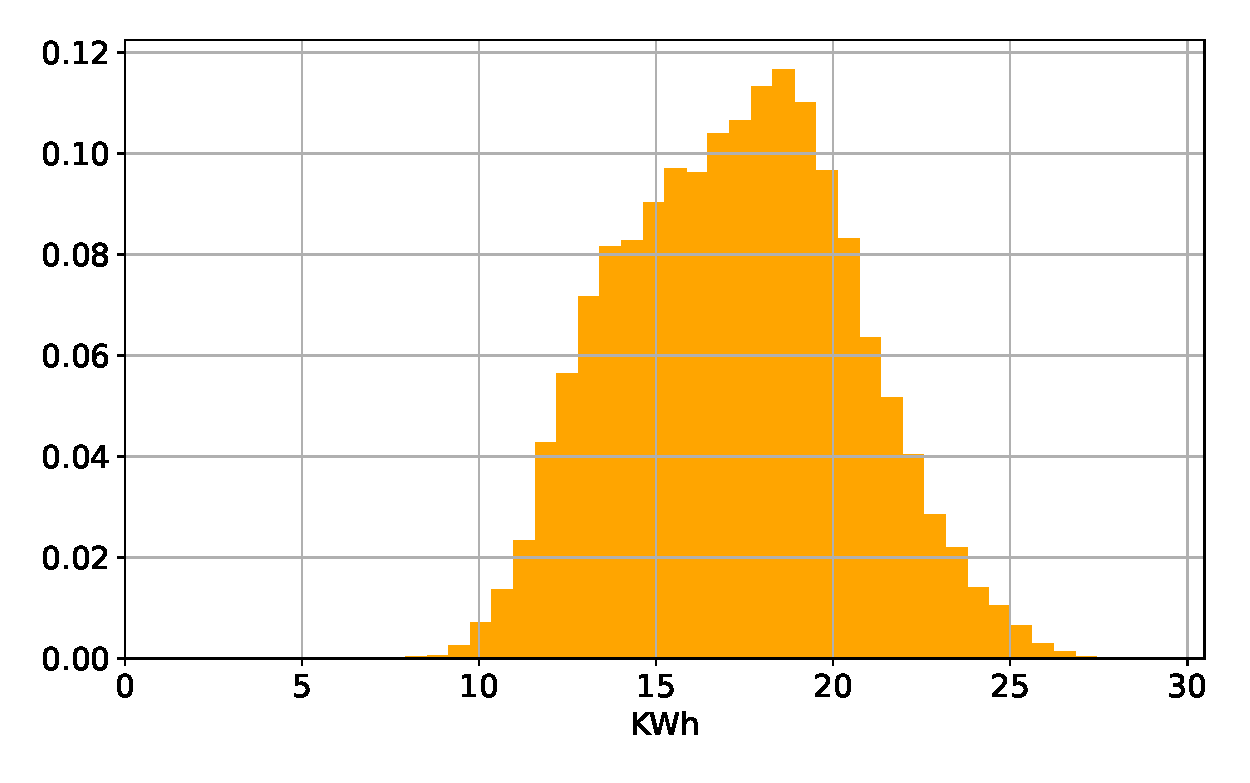
\includegraphics[width=0.295\textwidth]{histo_ej_pandeazucar} &
            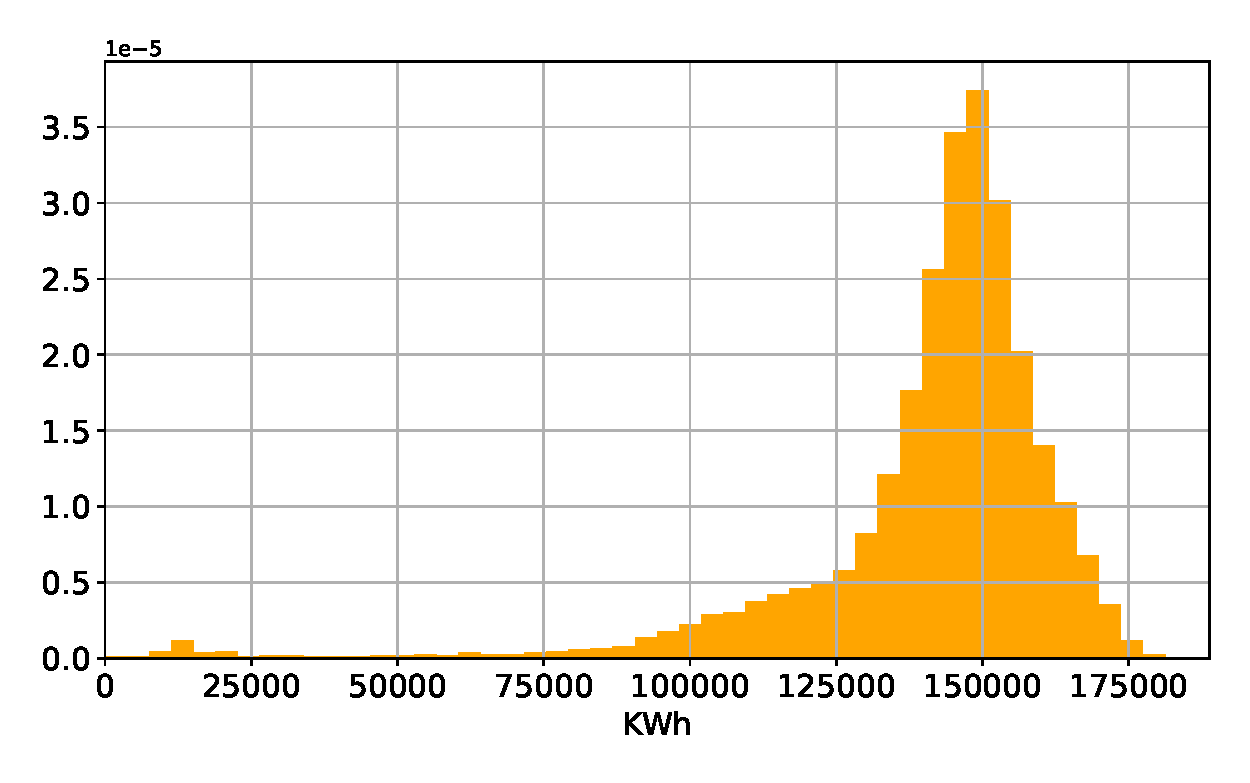
\includegraphics[width=0.295\textwidth]{histo_ej_quillota} &
            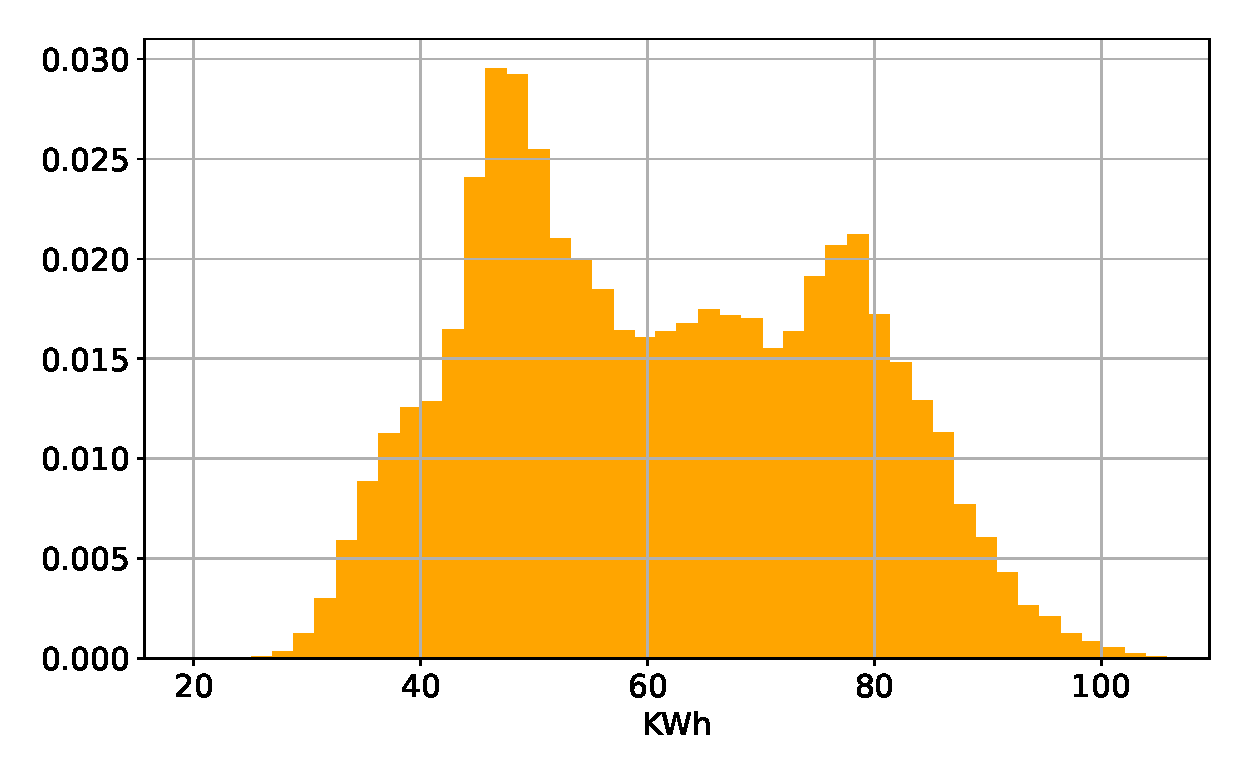
\includegraphics[width=0.295\textwidth]{histo_ej_sanjoaquin}
        \end{tabular}
    \end{center}
\end{frame}

\begin{frame}
    \frametitle{Histograma -- ejemplo demanda eléctrica}
    \begin{center}
        \begin{tabular}{cc}
            Datos originales & Aplicando logaritmo \\
            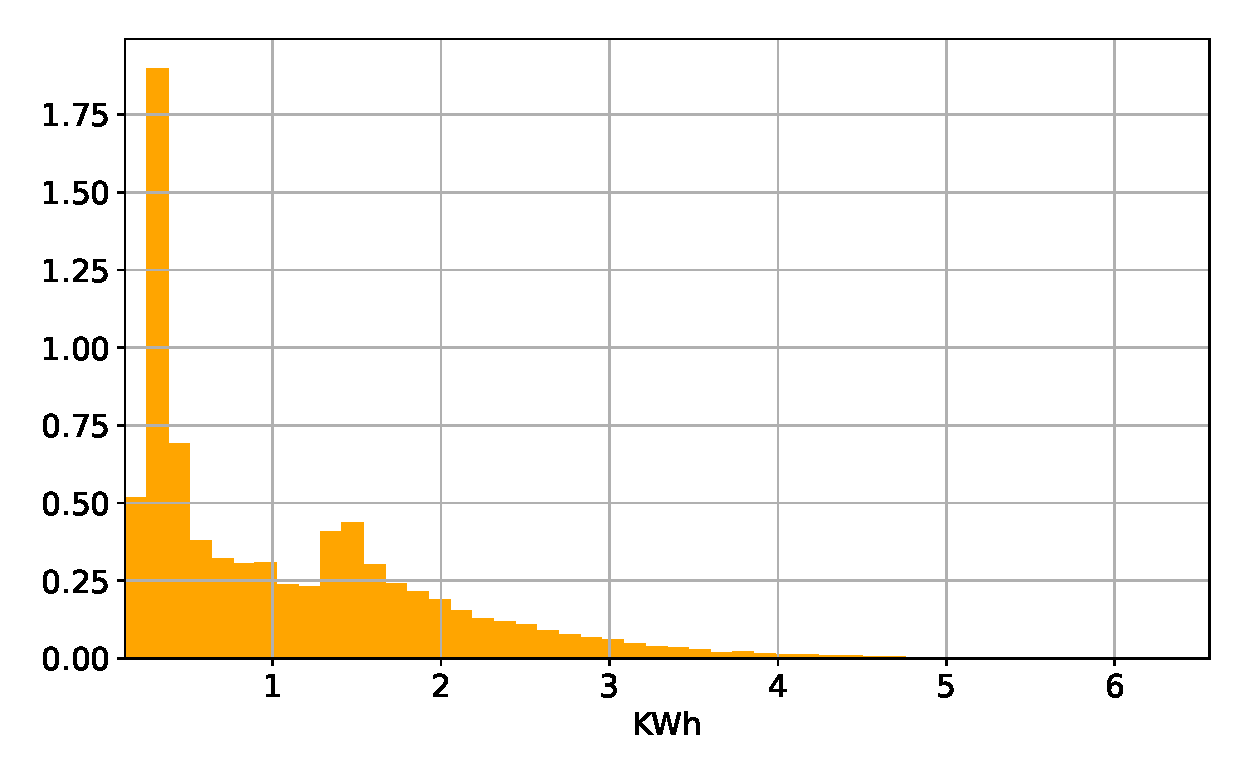
\includegraphics[width=0.46\textwidth]{histo_nolog} &
            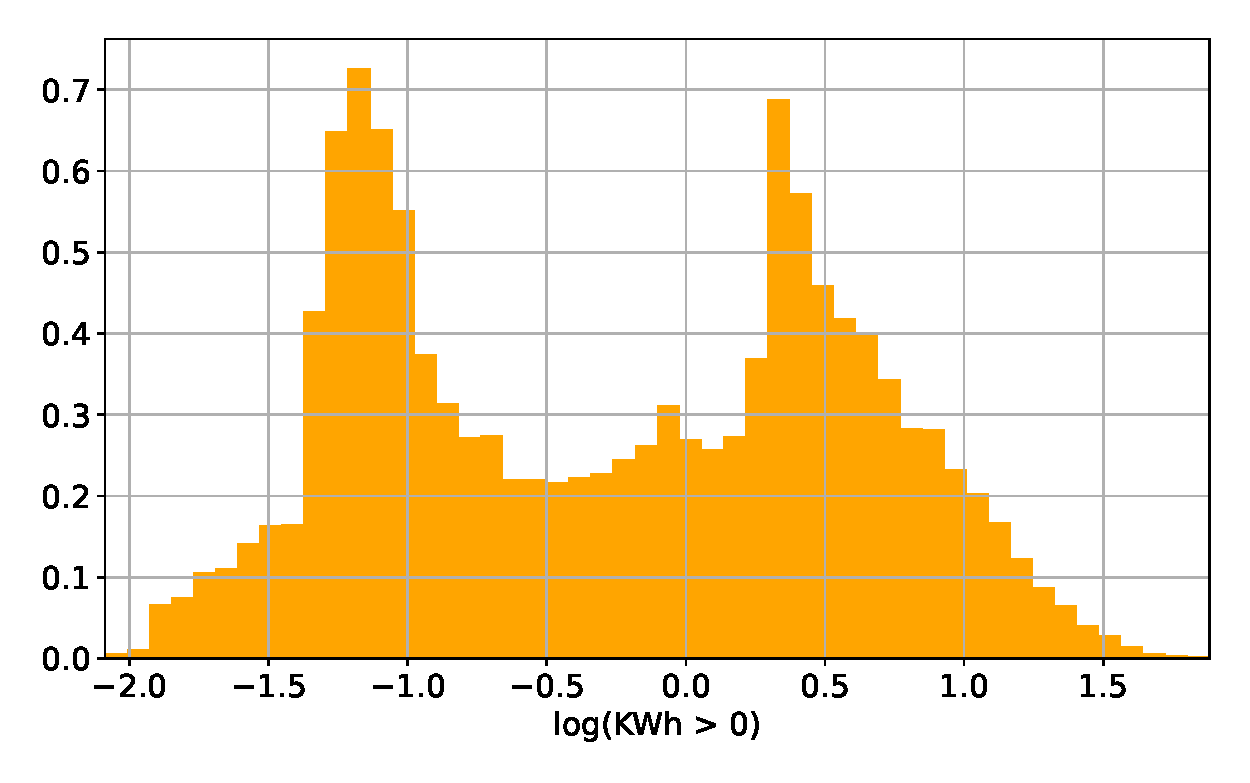
\includegraphics[width=0.46\textwidth]{histo_log}
        \end{tabular}
    \end{center}
\end{frame}

\begin{frame}
    \frametitle{Histograma -- polígono de frecuencias}
    \begin{center}
        \includegraphics[width=0.7\textwidth]{poligono_frecuencias}
    \end{center}
\end{frame}

\begin{frame}
    \frametitle{Histograma -- frecuencia acumulada}
    \begin{center}
        \includegraphics[width=0.49\textwidth]{frecuencia_acumulada}
        \includegraphics[width=0.49\textwidth]{frecuencia_acumulada_2}
    \end{center}
\end{frame}

\begin{frame}
    \frametitle{Histograma -- ¿cuántos intervalos?}
    \begin{center}
        \begin{tabular}{cc}
            \includegraphics[width=0.32\textwidth]{histo_bins2} &
            \includegraphics[width=0.32\textwidth]{histo_bins3} \\
            \includegraphics[width=0.32\textwidth]{histo_bins4} &
            \includegraphics[width=0.32\textwidth]{histo_bins5}
        \end{tabular}
    \end{center}
    \begin{alertblock}{Heurística: regla de Sturges}
        \begin{itemize}
            \item Se puede elegir cantidad $k = 1 + \log n$, donde $k$ es la cantidad de clases (intervalos) y $n$ la cantidad de datos.
            \item Recordar que \textbf{es solo una heurística}.
        \end{itemize}
    \end{alertblock}
\end{frame}

\begin{frame}
    \frametitle{Nota al margen -- Kernel Density Plot}
    \begin{center}
        \includegraphics[width=\textwidth]{kernel_density_plot}
    \end{center}
    \begin{alertblock}{Otros asuntos}
        \begin{itemize}
            \item Mezcla de gaussianas (normales).
            \item Ventanas de Parzen.
        \end{itemize}
    \end{alertblock}
\end{frame}

\begin{frame}
    \frametitle{Un ejemplo: palabras en libros en inglés}
    \begin{center}
        \includegraphics[height=0.86\textheight]{frecuencia_palabras_ingles}
    \end{center}
\end{frame}

\pgfplotstableread{
    name value
    1 0.05326117629142522
    2 0.2597032394622904
    3 0.12775800842612905
    4 0.06775726841855916
    5 0.09620279330275254
    6 0.08678590035632554
    7 0.09127309511987754
    8 0.07060362635108289
    9 0.05437460286416099
    10 0.038969254868325046
    11 0.022744711806365853
    12 0.012912971494628504
    13 0.008397404530133098
    14 0.0050476149706461535
    15+ 0.004208331737298012
}{\mytable}

\begin{frame}
    \frametitle{Preguntas}
    \begin{exampleblock}{Largo de palabras en castellano}
        \small
        ¿Con qué tipo de dato se está trabajando? ¿Qué significa que la frecuencia relativa de las palabras de largo $15$ o más sea $0.004$?
        \begin{center}
        \begin{tikzpicture}
            \begin{axis}[
                    tiny,
                    %title={Distribuci\'on de largos de palabras de wikipedia en español},
                    ylabel={Frec. relativa},
                    xlabel={Cantidad de letras},
                    width=0.8\textwidth,
                    height=0.3\textheight,
                    ymajorgrids,
                    ybar,
                    no markers,
                    xtick=data,
                    xticklabels from table={\mytable}{name},
                ]
                \addplot+[ybar] table[x expr=\coordindex] \mytable;
            \end{axis}
        \end{tikzpicture}
        \end{center}
    \end{exampleblock}
    \begin{exampleblock}{Horas de juego de juegos video}
        \small
        ¿Qué histograma considera más apropiado para explorar las propiedades de la cantidad de horas?
        \begin{center}
    \includegraphics[width=0.25\textwidth]{histo_control1_1}
    \includegraphics[width=0.25\textwidth]{histo_control1_2}
        \end{center}
    \end{exampleblock}
\end{frame}

\begin{frame}
    \frametitle{Medidas de localización}
    \begin{block}{Media muestral (media aritmética)}
        \begin{equation*}
            \bar{x} = \frac{x_{1} + x_{2} + \cdots + x_{n}}{n} = \frac{1}{n} \sum_{i = 1}^{n} x_{i} = \frac{\sum_{i = 1}^{n} x_{i}}{n}.
        \end{equation*}
        \begin{itemize}
            \item Busca estimar la \emph{media} de la población, denotada como $\mu$.
        \end{itemize}
    \end{block}
    \begin{exampleblock}{Ejemplo: temperaturas máximas durante enero}
        \begin{itemize}
            \item 22, 24, 21, 22, 25, 26, 25, 24, 23, 25, 25, 26, 27, 25, 26, 25, 26, 27, 27, 28, 29, 29, 29, 28, 30, 29, 30, 31, 30, 28, 29.
            \item $\bar{x} = \frac{22 + 24 + 21 + \cdots + 28 + 29}{31} = 26.48$ ºC.
        \end{itemize}
    \end{exampleblock}
\end{frame}

\begin{frame}
    \frametitle{Media muestral -- promedio}
    \begin{exampleblock}{Ejemplo: temperaturas máximas durante enero}
        \begin{itemize}
            \item 22, 24, 21, 22, 25, 26, 25, 24, 23, 25, 25, 26, 27, 25, 26, 25, 26, 27, 27, 28, 29, 29, 29, 28, 30, 29, 30, 31, 30, 28, 29.
        \end{itemize}
        \begin{center}
            \begin{tabular}{c|c|c|c|c}
                $< 20$ & $\left ( 20 , 25 \right ]$ & $\left ( 25 , 30 \right ]$ & $\left ( 30 , 35 \right ]$ & $> 35$ \\
                \hline
                $n_{1} = 0$ & $n_{2} = 12$ & $n_{3} = 18$ & $n_{4} = 1$ & $n_{5} = 0$ \\
                \hline
                $f_{1} = 0$ & $f_{2} = \frac{12}{31}$ & $f_{3} = \frac{18}{31}$ & $f_{4} = \frac{1}{31}$ & $f_{5} = 0$ \\
            \end{tabular}
            %\includegraphics[width=0.7\textwidth]{agrupados_media}
        \end{center}
    \end{exampleblock}
    \begin{block}{Datos agrupados}
        \begin{itemize}
            \item Se debe elegir \textbf{marca de clase} (representante de la clase).
            \item Ejemplo: valor medio de cada intervalo: $m_{j} = \frac{e_{j - 1} + e_{j}}{2}$.
            \item Media aritmética con pesos $\bar{x} = \frac{1}{n} \sum_{j = 1}^{k} n_{j} m_{j} = \sum_{j = 1}^{k} f_{j} m_{j}$.
            \item Ejemplo: $\bar{x} = 0 + \frac{12}{31} 22.5 + \frac{18}{31} 27.5 + \frac{1}{31} 32.5 + 0 \approx 25.7$ ºC.
        \end{itemize}
    \end{block}
\end{frame}

\begin{frame}
    \frametitle{Media muestral -- promedio}
    \begin{exampleblock}{Ejemplo: temperaturas máximas durante enero}
        \begin{itemize}
            \item 22, 24, 21, 22, 25, 26, 25, 24, 23, 25, 25, 26, 27, 25, 26, 25, 26, 27, 27, 28, 29, 29, 29, 28, 30, 29, 30, 31, 30, 28, 29.
        \end{itemize}
        \begin{center}
            \begin{tabular}{c|c|c|c|c}
                $< 20$ & $\left ( 20 , 25 \right ]$ & $\left ( 25 , 30 \right ]$ & $\left ( 30 , 35 \right ]$ & $> 35$ \\
                \hline
                $n_{1} = 0$ & $n_{2} = 12$ & $n_{3} = 18$ & $n_{4} = 1$ & $n_{5} = 0$ \\
                \hline
                $f_{1} = 0$ & $f_{2} = \frac{12}{31}$ & $f_{3} = \frac{18}{31}$ & $f_{4} = \frac{1}{31}$ & $f_{5} = 0$ \\
            \end{tabular}
            %\includegraphics[width=0.7\textwidth]{agrupados_media}
        \end{center}
    \end{exampleblock}
    \begin{block}{Datos agrupados}
        \begin{itemize}
            \item Para evitar el problema: media de medias.
                \begin{equation*}
                    \bar{x} = \frac{1}{n} \sum_{j = 1}^{k} n_{j} \bar{x}_{j} = \sum_{j = 1}^{k} f_{j} \bar{x}_{j} .
                \end{equation*}
            \item Ejemplo: $\bar{x} = 0 + \frac{12}{31} 23.83 + \frac{18}{31} 28 + \frac{1}{31} 31 + 0 = 26.48$ ºC.
        \end{itemize}
    \end{block}
\end{frame}

\begin{frame}
    \frametitle{Medidas de localización}
    \begin{block}{Mediana muestral}
        \begin{equation*}
            \tilde{x}_{0.5} =
            \begin{cases}
                x_{\parens{\frac{n + 1}{2}}} \text{ si } n \text{ es impar} , \\
                \frac{1}{2} \parens{x_{\parens{\frac{n}{2}}} + x_{\parens{\frac{n}{2} + 1}}} \text{ si } n \text{ es par} .
            \end{cases}
        \end{equation*}
        \begin{itemize}
            \item $x_{i}$ observación $i$-ésima.
            \item $x_{\parens{i}}$ estadística de orden $i$-ésima.
            \item $x_{\parens{1}} = \min \bparens{x_{i}}_{i = 1}^{n}$ y $x_{\parens{n}} = \max \bparens{x_{i}}_{i = 1}^{n}$.
        \end{itemize}
    \end{block}
    \begin{exampleblock}{Ejemplo: temperaturas máximas durante enero}
            \begin{center}
                \footnotesize
                \begin{tabular}{cccccccccccccccc}
                    21 & 22 & 22 & 23 & 24 & 24 & 25 & 25 & 25 & 25 & 25 & 25 & 26 & 26 & 26 & 26 \\
                    1 & 2 & 3 & 4 & 5 & 6 & 7 & 8 & 9 & 10 & 11 & 12 & 13 & 14 & 15 & 16 \\
                    \hline
                    27 & 27 & 27 & 28 & 28 & 28 & 29 & 29 & 29 & 29 & 29 & 30 & 30 & 30 & 31 & \\
                    17 & 18 & 19 & 20 & 21 & 22 & 23 & 24 & 25 & 26 & 27 & 28 & 29 & 30 & 31 & \\
                \end{tabular}
                %\includegraphics[width=0.8\textwidth]{mediana_ej}
            \end{center}
        \begin{itemize}
            \item $\tilde{x}_{0.5} = 26$ ºC.
        \end{itemize}
    \end{exampleblock}
\end{frame}

\begin{frame}
    \frametitle{Mediana muestral -- datos agrupados}
    \begin{exampleblock}{Ejemplo: temperaturas máximas durante enero}
        \begin{itemize}
            \item 22, 24, 21, 22, 25, 26, 25, 24, 23, 25, 25, 26, 27, 25, 26, 25, 26, 27, 27, 28, 29, 29, 29, 28, 30, 29, 30, 31, 30, 28, 29.
        \end{itemize}
        \begin{center}
            \begin{tabular}{c|c|c|c|c}
                $< 20$ & $\left ( 20 , 25 \right ]$ & $\left ( 25 , 30 \right ]$ & $\left ( 30 , 35 \right ]$ & $> 35$ \\
                \hline
                $n_{1} = 0$ & $n_{2} = 12$ & $n_{3} = 18$ & $n_{4} = 1$ & $n_{5} = 0$ \\
                \hline
                $f_{1} = 0$ & $f_{2} = \frac{12}{31}$ & $f_{3} = \frac{18}{31}$ & $f_{4} = \frac{1}{31}$ & $f_{5} = 0$ \\
            \end{tabular}
            %\includegraphics[width=0.7\textwidth]{agrupados_media}
        \end{center}
    \end{exampleblock}
    \begin{block}{Datos agrupados}
        \begin{itemize}
            \item Clase $m$ es la clase que cumple que $\sum_{j = 1}^{m - 1} f_{j} < 0.5$ y $\sum_{j = 1}^{m} f_{j} \geq 0.5$.
            \item Mediana interpolada $\tilde{x}_{0.5} = e_{m - 1} + \frac{0.5 - \sum_{j = 1}^{m - 1} f_{j}}{f_{m}} \parens{e_{m} - e_{m - 1}}.$
            \item Ejemplo: $\tilde{x}_{0.5} = 25 + \frac{0.5 - \frac{12}{31}}{\frac{18}{31}} 5 \approx 25.97$ ºC.
        \end{itemize}
    \end{block}
\end{frame}

\begin{frame}
    \frametitle{Media vs mediana}
    \begin{center}
        \begin{tabular}{cc}
            Simétricos & Asimétricos \\
            \includegraphics[width=0.28\textwidth]{media_mediana1} &
            \includegraphics[width=0.28\textwidth]{media_mediana2} \\
            Bimodales & Valores atípicos / extremos \\
            \includegraphics[width=0.28\textwidth]{media_mediana3} &
            \includegraphics[width=0.28\textwidth]{media_mediana4}
        \end{tabular}
    \end{center}
\end{frame}

\begin{frame}
    \frametitle{Generalización de la mediana}
    \begin{block}{Cuantiles}
        \begin{equation*}
            \tilde{x}_{\alpha} =
            \begin{cases}
                x_{\parens{\left \lceil n \alpha \right \rceil}} \text{ si } n \alpha \text{ no es entero} , \\
                \frac{1}{2} \parens{x_{\parens{n \alpha}} + x_{\parens{n \alpha + 1}}} \text{ si } n \alpha \text{ es entero} .
            \end{cases}
        \end{equation*}
        \begin{itemize}
            \item ¿Es la única manera de interpolar?
        \end{itemize}
    \end{block}
    \begin{exampleblock}{Ejemplo: temperaturas máximas durante enero}
            \begin{center}
                \footnotesize
                \begin{tabular}{cccccccccccccccc}
                    21 & 22 & 22 & 23 & 24 & 24 & 25 & 25 & 25 & 25 & 25 & 25 & 26 & 26 & 26 & 26 \\
                    1 & 2 & 3 & 4 & 5 & 6 & 7 & 8 & 9 & 10 & 11 & 12 & 13 & 14 & 15 & 16 \\
                    \hline
                    27 & 27 & 27 & 28 & 28 & 28 & 29 & 29 & 29 & 29 & 29 & 30 & 30 & 30 & 31 & \\
                    17 & 18 & 19 & 20 & 21 & 22 & 23 & 24 & 25 & 26 & 27 & 28 & 29 & 30 & 31 & \\
                \end{tabular}
                %\includegraphics[width=0.8\textwidth]{mediana_ej}
            \end{center}
        \begin{itemize}
            %\item 22, 24, 21, 22, 25, 26, 25, 24, 23, 25, 25, 26, 27, 25, 26, 25, 26, 27, 27, 28, 29, 29, 29, 28, 30, 29, 30, 31, 30, 28, 29.
            \item $\tilde{x}_{0.25} = x_{\parens{\left \lceil 7 \frac{3}{4} \right \rceil}} = x_{\parens{8}} = 25$ ºC.
            \item $\tilde{x}_{0.5} = x_{\parens{\left \lceil 15 \frac{1}{2} \right \rceil}} = x_{\parens{16}} = 26$ ºC.
            \item $\tilde{x}_{0.75} = x_{\parens{\left \lceil 23 \frac{1}{4} \right \rceil}} = x_{\parens{24}} = 29$ ºC.
        \end{itemize}
    \end{exampleblock}
\end{frame}

\begin{frame}
    \frametitle{Cuantiles y frecuencia acumulada}
    \begin{center}
        \includegraphics[width=0.7\textwidth]{frecuencia_acumulada}
    \end{center}
    \begin{block}{}
        \begin{itemize}
            \item Deciles, quintiles, cuartiles, etc.
        \end{itemize}
    \end{block}
\end{frame}

\begin{frame}
    \frametitle{Medidas de dispersión / variabilidad}
    \begin{block}{Rango}
        \begin{itemize}
            \item $R = x_{\parens{n}} - x_{\parens{1}} = \max \bparens{x_{i}}_{i = 1}^{n} - \min \bparens{x_{i}}_{i = 1}^{n}$.% = \max_{i \in \bparens{1 , \ldots , n}} x_{i} - \min_{i \in \bparens{1 , \ldots , n}} x_{i}$.
            %\item El máximo menos el mínimo.
        \end{itemize}
    \end{block}
    \begin{block}{Rango intercuantil}
        \begin{itemize}
            \item ${Q}_{\alpha} = \tilde{x}_{\frac{1 + \alpha}{2}} - \tilde{x}_{\frac{1 - \alpha}{2}}$.
            \item Ejemplo: intercuartil $\alpha = 0.5$: $Q_{0.5} = \tilde{x}_{0.75} - \tilde{x}_{0.25}$.
        \end{itemize}
    \end{block}
        % \includegraphics[width=0.7\textwidth]{mediana_ej}
    \begin{exampleblock}{Ejemplo: temperaturas máximas durante enero}
        \begin{center}
                \footnotesize
                \begin{tabular}{cccccccccccccccc}
                    21 & 22 & 22 & 23 & 24 & 24 & 25 & 25 & 25 & 25 & 25 & 25 & 26 & 26 & 26 & 26 \\
                    1 & 2 & 3 & 4 & 5 & 6 & 7 & 8 & 9 & 10 & 11 & 12 & 13 & 14 & 15 & 16 \\
                    \hline
                    27 & 27 & 27 & 28 & 28 & 28 & 29 & 29 & 29 & 29 & 29 & 30 & 30 & 30 & 31 & \\
                    17 & 18 & 19 & 20 & 21 & 22 & 23 & 24 & 25 & 26 & 27 & 28 & 29 & 30 & 31 & \\
                \end{tabular}
                %\includegraphics[width=0.8\textwidth]{mediana_ej}
        \end{center}
        \begin{itemize}
            \item $R = 31 - 21 = 10$ ºC.
            \item $Q_{0.5} = 29 - 25 = 4$ ºC.
        \end{itemize}
    \end{exampleblock}
\end{frame}

\begin{frame}
    \frametitle{Gráfico de caja (\emph{boxplot})}
    \begin{center}
        \begin{tikzpicture}[thick,scale=0.8, every node/.style={scale=0.6}]
            \begin{axis}[
                boxplot/draw direction=y,
                %small,
                %footnotesize,
                %clip=false,
                %domain=-2:2,
                %samples=50,
                %legend entries={$x$\\$x^{2}$\\$x^{3}$\\$x^{4}$\\},
                %legend pos=south east,
                %legend style={font=\footnotesize},
                %height=0.5\textheight,
                %axis lines=middle,
                %xtick=\empty,
                hide x axis=true,
                ymajorgrids,
                width=0.95\textwidth,
                height=0.65\textheight,
                xmin=0,%-0.5,
                xmax=3,%3.5,
                %ymin=-0.2,
                %ymax=10.5,
                %grid=major,
                %no markers,
                ]
                \addplot+ [
                    thick,
                    boxplot prepared={
                        lower whisker=0,
                        lower quartile=1,
                        median=2,
                        upper quartile=4,
                        upper whisker=10,
                        },
                    ] coordinates {};
                \addplot+ [
                    thick,
                    mark=*,
                    boxplot prepared={
                        lower whisker=1.5,
                        lower quartile=3.3,
                        median=4,
                        upper quartile=4.5,
                        upper whisker=6.3,
                        },
                    ]
                    table [row sep=\\,y index=0] {
                        0\\ 0.8\\ 0.95\\ 7.5\\ 8\\ 8.5\\ 8.6\\ 8.7\\ 10\\
                    };
                \node[pin=175:Mediana $\tilde{x}_{0.5}$] at (axis cs:0.70,2) {};
                \node[pin=130:3er cuartil $\tilde{x}_{0.75}$] at (axis cs:0.95,4) {};
                \node[pin=200:1er cuartil $\tilde{x}_{0.25}$] at (axis cs:0.98,0.5) {};
                \node[pin=5:$\tilde{x}_{0.75} + 1.5 Q_{0.5}$] at (axis cs:2,6.3) {};
                \node[pin=5:$\tilde{x}_{0.25} - 1.5 Q_{0.5}$] at (axis cs:2,1.5) {};
            \end{axis}
        \end{tikzpicture}
        %\includegraphics[width=0.9\textwidth]{boxplot}
    \end{center}
    \begin{block}{Valores atípicos / extremos (\emph{outliers})}
        \begin{itemize}
            \item $Q_{0.5} = \tilde{x}_{0.75} - \tilde{x}_{0.25}$.
            \item $x_{i}$ valor atípico si $x_{i} - \tilde{x}_{0.75} > 1.5 Q_{0.5}$, o si
                $\tilde{x}_{0.25} - x_{i} > 1.5 Q_{0.5}$.
            \item $x_{i}$ valor extremo si $x_{i} - \tilde{x}_{0.75} > 3 Q_{0.5}$, o si
                $\tilde{x}_{0.25} - x_{i} > 3 Q_{0.5}$.
            \item Estas definiciones varían según libro, biblioteca, etc. Es configurable.
        \end{itemize}
    \end{block}
\end{frame}

\begin{frame}
    \frametitle{Asimetría (\emph{skewness})}
    \begin{block}{Coeficiente/índice de Bowley / Yule}
        \begin{equation*}
            \frac{\parens{\tilde{x}_{0.75} - \tilde{x}_{0.5}} - \parens{\tilde{x}_{0.5} - \tilde{x}_{0.25}}}{\tilde{x}_{0.75} - \tilde{x}_{0.25}}
            = \frac{\tilde{x}_{0.25} + \tilde{x}_{0.75} - 2 \tilde{x}_{0.5}}{\tilde{x}_{0.75} - \tilde{x}_{0.25}} .
        \end{equation*}
    \end{block}
    \begin{center}
        \begin{tikzpicture}[thick,scale=0.9, every node/.style={scale=0.7}]
            \begin{axis}[
                boxplot/draw direction=y,
                %small,
                %footnotesize,
                %clip=false,
                %domain=-2:2,
                %samples=50,
                %legend entries={$x$\\$x^{2}$\\$x^{3}$\\$x^{4}$\\},
                %legend pos=south east,
                %legend style={font=\footnotesize},
                %height=0.5\textheight,
                %axis lines=middle,
                %xtick=\empty,
                hide x axis=true,
                ymajorgrids,
                width=0.95\textwidth,
                height=0.65\textheight,
                xmin=0,%-0.5,
                xmax=3,%3.5,
                %ymin=-0.2,
                %ymax=10.5,
                %grid=major,
                %no markers,
                ]
                \addplot+ [
                    thick,
                    boxplot prepared={
                        lower whisker=0,
                        lower quartile=1,
                        median=2,
                        upper quartile=4,
                        upper whisker=10,
                        },
                    ] coordinates {};
                \addplot+ [
                    thick,
                    mark=*,
                    boxplot prepared={
                        lower whisker=1.5,
                        lower quartile=3.3,
                        median=4,
                        upper quartile=4.5,
                        upper whisker=6.3,
                        },
                    ]
                    table [row sep=\\,y index=0] {
                        0\\ 0.8\\ 0.95\\ 7.5\\ 8\\ 8.5\\ 8.6\\ 8.7\\ 10\\
                    };
                \node[pin=175:Mediana $\tilde{x}_{0.5}$] at (axis cs:0.75,2) {};
                \node[pin=130:3er cuartil $\tilde{x}_{0.75}$] at (axis cs:0.95,4) {};
                \node[pin=200:1er cuartil $\tilde{x}_{0.25}$] at (axis cs:0.98,0.6) {};
                \node[pin=5:$\tilde{x}_{0.75} + 1.5 Q_{0.5}$] at (axis cs:2,6.3) {};
                \node[pin=5:$\tilde{x}_{0.25} - 1.5 Q_{0.5}$] at (axis cs:2,1.5) {};
            \end{axis}
        \end{tikzpicture}
        %\includegraphics[width=0.9\textwidth]{boxplot}
    \end{center}
\end{frame}

\begin{frame}
    \frametitle{Medidas de localización}
    \begin{block}{Moda}
        \begin{itemize}
            \item El valor más frecuente.
            \item Puede haber más de un valor modal.
        \end{itemize}
    \end{block}
        % \includegraphics[width=0.8\textwidth]{mediana_ej}
    \begin{exampleblock}{Ejemplo: temperaturas máximas durante enero}
        \begin{itemize}
            \item 22, 24, 21, 22, 25, 26, 25, 24, 23, 25, 25, 26, 27, 25, 26, 25, 26, 27, 27, 28, 29, 29, 29, 28, 30, 29, 30, 31, 30, 28, 29.
        \end{itemize}
            \begin{center}
                \footnotesize
                \begin{tabular}{cccccccccccccccc}
                    21 & 22 & 22 & 23 & 24 & 24 & 25 & 25 & 25 & 25 & 25 & 25 & 26 & 26 & 26 & 26 \\
                    1 & 2 & 3 & 4 & 5 & 6 & 7 & 8 & 9 & 10 & 11 & 12 & 13 & 14 & 15 & 16 \\
                    \hline
                    27 & 27 & 27 & 28 & 28 & 28 & 29 & 29 & 29 & 29 & 29 & 30 & 30 & 30 & 31 & \\
                    17 & 18 & 19 & 20 & 21 & 22 & 23 & 24 & 25 & 26 & 27 & 28 & 29 & 30 & 31 & \\
                \end{tabular}
                %\includegraphics[width=0.8\textwidth]{mediana_ej}
            \end{center}
        \begin{itemize}
            \item Moda $= 25$ ºC.
        \end{itemize}
    \end{exampleblock}
\end{frame}

\begin{frame}
    \frametitle{Moda -- datos agrupados}
    \begin{block}{Moda}
        \begin{itemize}
            \item El intervalo / clase más frecuente.
            \item ¿Cuál es su representante?
        \end{itemize}
    \end{block}
        %\includegraphics[width=0.7\textwidth]{agrupados_media}
    \begin{exampleblock}{Ejemplo: temperaturas máximas durante enero}
        \begin{itemize}
            \item 22, 24, 21, 22, 25, 26, 25, 24, 23, 25, 25, 26, 27, 25, 26, 25, 26, 27, 27, 28, 29, 29, 29, 28, 30, 29, 30, 31, 30, 28, 29.
        \end{itemize}
        \begin{center}
            \begin{tabular}{c|c|c|c|c}
                $< 20$ & $\left ( 20 , 25 \right ]$ & $\left ( 25 , 30 \right ]$ & $\left ( 30 , 35 \right ]$ & $> 35$ \\
                \hline
                $n_{1} = 0$ & $n_{2} = 12$ & $n_{3} = 18$ & $n_{4} = 1$ & $n_{5} = 0$ \\
                \hline
                $f_{1} = 0$ & $f_{2} = \frac{12}{31}$ & $f_{3} = \frac{18}{31}$ & $f_{4} = \frac{1}{31}$ & $f_{5} = 0$ \\
            \end{tabular}
            %\includegraphics[width=0.7\textwidth]{agrupados_media}
        \end{center}
        \begin{itemize}
            \item Clase modal es intervalo $( 25 , 30 ]$ ºC.
        \end{itemize}
    \end{exampleblock}
\end{frame}

\begin{frame}
    \frametitle{Medidas de dispersión / variabilidad / volatilidad}
    \begin{block}{Desviación absoluta}
        \begin{equation*}
            D \parens{A} = \frac{1}{n} \sum_{i = 1}^{n} \vparens{x_{i} - A} .
        \end{equation*}
    \end{block}
    \begin{exampleblock}{Ejemplo: desviación absoluta de la media}
        \begin{equation*}
            D \parens{\bar{x}} = \frac{1}{n} \sum_{i = 1}^{n} \vparens{x_{i} - \bar{x}} .
        \end{equation*}
    \end{exampleblock}
    \begin{block}{Mínimo: se obtiene con la mediana $\tilde{x}_{0.5}$}
        \begin{equation*}
            D \parens{\tilde{x}_{0.5}} = \frac{1}{n} \sum_{i = 1}^{n} \vparens{x_{i} - \tilde{x}_{0.5}} .
        \end{equation*}
    \end{block}
\end{frame}

\begin{frame}
    \frametitle{Medidas de dispersión / variabilidad / volatilidad}
    \begin{block}{Error cuadrático medio}
        \begin{equation*}
            s^{2} \parens{A} = \frac{1}{n} \sum_{i = 1}^{n} \parens{x_{i} - A}^{2} .
        \end{equation*}
    \end{block}
    \begin{block}{Mínimo: se obtiene con la media $\bar{x}$, y a su valor se le llama varianza}
        \begin{equation*}
            s^{2} \parens{\bar{x}} = \frac{1}{n} \sum_{i = 1}^{n} \parens{x_{i} - \bar{x}}^{2}
            = \frac{1}{n} \sum_{i = 1}^{n} \parens{x_{i}^{2} - \bar{x}^{2}}
            = \parens{\frac{1}{n} \sum_{i = 1}^{n} x_{i}^{2}} - \bar{x}^{2} .
        \end{equation*}
    \end{block}
    \begin{block}{Varianza muestral}
        \begin{itemize}
            \item $\bar{x}$ es una estimación de $\mu$, la media de la población.
        \end{itemize}
        \begin{equation*}
            s^{2} = \frac{1}{n - 1} \sum_{i = 1}^{n} \parens{x_{i} - \bar{x}}^{2}
            = \frac{1}{n - 1} \sum_{i = 1}^{n} x_{i}^{2} - \frac{n}{n - 1} \bar{x}^{2} .
        \end{equation*}
        \begin{itemize}
            \item Desviación estándar: $s = \sqrt{s^{2}}$.
        \end{itemize}
    \end{block}
\end{frame}

\begin{frame}
    \frametitle{Varianza -- desviación estándar}
    \begin{block}{Datos agrupados / Datos muestrales}
        \begin{equation*}
            s^{2} \approx \frac{1}{n - 1} \sum_{j = 1}^{k} n_{j} \parens{m_{j} - \bar{x}}^{2}
            \approx \frac{n}{n - 1} \sum_{j = 1}^{k} f_{j} \parens{m_{j} - \bar{x}}^{2} .
        \end{equation*}
        \begin{equation*}
            s^{2} \approx \frac{1}{n - 1} \sum_{j = 1}^{k} n_{j} \parens{\bar{x}_{j} - \bar{x}}^{2}
            \approx \frac{n}{n - 1} \sum_{j = 1}^{k} f_{j} \parens{\bar{x}_{j} - \bar{x}}^{2} .
        \end{equation*}
    \end{block}
    \begin{exampleblock}{Ejemplo: temperaturas máximas durante enero}
        \begin{center}
            \begin{tabular}{c|c|c|c|c}
                $< 20$ & $\left ( 20 , 25 \right ]$ & $\left ( 25 , 30 \right ]$ & $\left ( 30 , 35 \right ]$ & $> 35$ \\
                \hline
                $n_{1} = 0$ & $n_{2} = 12$ & $n_{3} = 18$ & $n_{4} = 1$ & $n_{5} = 0$ \\
                \hline
                $f_{1} = 0$ & $f_{2} = \frac{12}{31}$ & $f_{3} = \frac{18}{31}$ & $f_{4} = \frac{1}{31}$ & $f_{5} = 0$ \\
            \end{tabular}
            %\includegraphics[width=0.7\textwidth]{agrupados_media}
        \end{center}
    \end{exampleblock}
\end{frame}

\begin{frame}
    \frametitle{Nota al margen -- varianza entre - intra clases}
    \begin{block}{Clase $j$}
        \begin{itemize}
            \item Media $\bar{x}_{j} = \frac{1}{n_{j}} \sum_{i \in \text{Clase } j} x_{i}$, varianza $s^{2}_{j} = \frac{1}{n} \sum_{i \in \text{Clase } j} \parens{x_{i} - \bar{x}_{j}}^{2}$.
        \end{itemize}
    \end{block}
    \begin{center}
        \begin{tabular}{c||c|c|c|c|c}
            Intervalo & $< 20$ & $\left ( 20 , 25 \right ]$ & $\left ( 25 , 30 \right ]$ & $\left ( 30 , 35 \right ]$ & $> 35$ \\
            \hline
            $n_{j}$ & $n_{1} = 0$ & $n_{2} = 12$ & $n_{3} = 18$ & $n_{4} = 1$ & $n_{5} = 0$ \\
            \hline
            $\bar{x}_{j}$ & -- & $23.83$ & $28$ & $31$ & -- \\
            $s^{2}_{j}$ & -- & $1.972$ & $2$ & $0$ & -- \\
        \end{tabular}
        %\includegraphics[width=0.8\textwidth]{agrupados_vars}
    \end{center}
    \begin{block}{Varianza entre clases e intra clases}
        \begin{equation*}
            s^{2} = \sparens{\frac{1}{n} \sum_{j = 1}^{k} n_{j} \parens{\bar{x}_{j} - \bar{x}}^{2}} + \sparens{\frac{1}{n} \sum_{j = 1}^{k} n_{j} s^{2}_{j}} .
        \end{equation*}
        \begin{itemize}
            \item $\frac{1}{31} \parens{12 \sparens{23.83 - 26.48}^{2} + 18 \sparens{28 - 26.48}^{2} + 1 \sparens{31 - 26.48}^{2}} + \frac{1}{31} \parens{12 \cdot 1.972 + 18 \cdot 2 + 1 \cdot 0} \approx 4.71 + 1.925$ .
        \end{itemize}
    \end{block}
\end{frame}

\begin{frame}
    \frametitle{Nota al margen -- varianza entre - intra clases}
    \begin{block}{Varianza entre clases e intra clases}
        \begin{equation*}
            s^{2} = \sparens{\frac{1}{n} \sum_{j = 1}^{k} n_{j} \parens{\bar{x}_{j} - \bar{x}}^{2}} + \sparens{\frac{1}{n} \sum_{j = 1}^{k} n_{j} s^{2}_{j}} .
        \end{equation*}
    \end{block}
    \begin{center}
        \includegraphics[width=0.5\textwidth]{within_between_variance}
    \end{center}
\end{frame}

\begin{frame}
    \frametitle{Algunas propiedades}
    \begin{block}{Transformaciones lineales $y_{i} = a + b x_{i}$}
        \begin{itemize}
            \item $\bar{y} = a + b \bar{x}$.
            \item $s^{2}_{y} = b^{2} s^{2}_{x}$.
            \item $s_{y} = \vparens{b} s_{x}$.
        \end{itemize}
    \end{block}
    \begin{exampleblock}{Ejemplo: estandarización}
        \begin{equation*}
            y_{i} = \frac{x_{i} - \bar{x}}{s_{x}} .
        \end{equation*}
        \begin{itemize}
            \item $\bar{y} = 0$, $s_{y} = 1$.
        \end{itemize}
    \end{exampleblock}
    \begin{alertblock}{Otras transformaciones}
        \begin{itemize}
            \item $y_{i} = a x_{i}^{2}$, $y_{i} = a \sqrt{x_{i}}$.
            \item $y_{i} = \ln x_{i}$.
            %\item $y_{i} = \ln \frac{x_{i + 1} - x_{i}}{x_{i}}$.
        \end{itemize}
    \end{alertblock}
\end{frame}

\begin{frame}
    \frametitle{Medidas de dispersión / variabilidad}
    \begin{block}{Coeficiente de variación}
        \begin{equation*}
            v = \frac{s}{\bar{x}}
        \end{equation*}
        \begin{itemize}
            \item Solo para valores positivos de razón.
            \item Permite comparar poblaciones con unidades diferentes, ya que si $y_{i} = b x_{i}$, se cumple que $v_{y} = \frac{s_{y}}{\bar{y}} = \frac{b s_{x}}{b \bar{x}} = \frac{s_{x}}{\bar{x}} = v_{x}$.
            \item A $\frac{\bar{x}}{s}$ se le llama \emph{razón señal ruido}.
        \end{itemize}
    \end{block}
    \begin{center}
        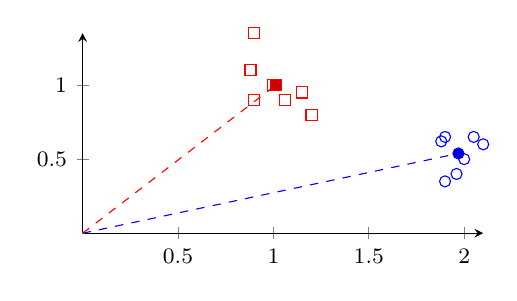
\begin{tikzpicture}
            \begin{axis}[
                small,
                width=0.55\textwidth,
                height=0.55\textwidth/1.618,
                axis lines=middle,
                xmin=0,
                ymin=0,
                ]
                \addplot+[only marks, forget plot, mark=o] coordinates {(2, 0.5) (2.1, 0.6) (2.05, 0.65) (1.9, 0.65) (1.88, 0.62) (1.9, 0.35) (1.96, 0.4)};
                \addplot+[dashed, forget plot, no markers] coordinates {(0, 0) (1.97, 0.538571429)};
                \addplot+[only marks, mark=*] coordinates {(1.97, 0.538571429)};
                \addplot+[only marks, forget plot, mark=square] coordinates {(1, 1) (1.2, 0.8) (1.15, 0.95) (0.9, 0.9) (0.88, 1.1) (0.9, 1.35) (1.06, 0.9)};
                \addplot+[dashed, forget plot, no markers] coordinates {(0, 0) (1.012857143, 1)};
                \addplot+[only marks, mark=square*] coordinates {(1.012857143, 1)};
            \end{axis}
        \end{tikzpicture}
        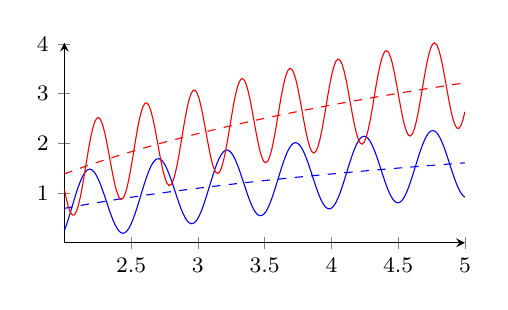
\begin{tikzpicture}
            \begin{axis}[
                small,
                width=0.55\textwidth,
                height=0.55\textwidth/1.618,
                samples=200,
                domain=2:5,
                axis lines=middle,
                no markers,
                ymin=0,
                ]
                \addplot+[dashed, forget plot] {ln(x)};
                \addplot+ {ln(x) + 0.7 * sin(700 * x)};
                \addplot+[dashed, forget plot] {2 * ln(x)};
                \addplot+ {2 * ln(x) + 0.9 * sin(1000 * x)};
            \end{axis}
        \end{tikzpicture}
    \end{center}
\end{frame}

\begin{frame}
    \frametitle{Otras medidas: momentos}
    \begin{block}{No centrados}
                \begin{equation*}
                    m_{k} = \frac{1}{n} \sum_{i = 1}^{n} x_{i}^{k}
                \end{equation*}
    \end{block}
    \begin{block}{Centrados}
                \begin{equation*}
                    \bar{m}_{k} = \frac{1}{n} \sum_{i = 1}^{n} \parens{x_{i} - m_{1}}^{k}
                \end{equation*}
    \end{block}
   % \begin{exampleblock}{Example}
   %         $m_{1} = \bar{x}$.
   % \end{exampleblock}
    \begin{center}
        \begin{tikzpicture}[thick,scale=0.9, every node/.style={scale=0.7}]
            \begin{axis}[
                small,
                clip=false,
                domain=-2:2,
                samples=50,
                legend entries={$x$\\$x^{2}$\\$x^{3}$\\$x^{4}$\\},
                legend pos=south east,
                legend style={font=\footnotesize},
                height=0.5\textheight,
                axis lines=middle,
                grid=major,
                no markers,
                ]
                \addplot+[thick] {x};
                \addplot+[thick, domain=-1.414213562:1.414213562] {x * x};
                \addplot+[thick, domain=-1.25992105:1.25992105] {x * x * x};
                \addplot+[thick, domain=-1.189207115:1.189207115] {x * x * x * x};
            \end{axis}
        \end{tikzpicture}
        %\includegraphics[width=0.34\textwidth]{exponente_momentos}
    \end{center}
\end{frame}

\begin{frame}
    \frametitle{Tercer momento: asimetría (\emph{skewness})}
    \begin{block}{Coeficiente de Fisher}
        \begin{equation*}
            \frac{\bar{m}_{3}}{s^{3}} .
        \end{equation*}
    \end{block}
    \begin{center}
        \begin{tabular}{ccc}
        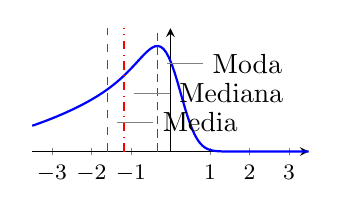
\begin{tikzpicture}[
            declare function={
                normal(\x,\m,\s) = 1 / (\s * sqrt(2 * pi)) * exp(-(\x - \m)^2 / (2 * \s^2));
                asinh(\x) = ln(\x + sqrt((\x^2) + 1));
                basex(\x,\m,\s) = (\x - \m) / \s;
                bigh(\x,\m,\s,\e,\d) = sinh(\d * asinh(basex(\x, \m, \s)) - \e);
                smallh(\x,\m,\s,\e,\d) = \d * cosh(\d * asinh(basex(\x, \m, \s)) - \e) / (\s * sqrt(2 * pi * (1 + ((basex(\x, \m, \s))^2))));
                sinhdist(\x,\m,\s,\e,\d) = smallh(\x, \m, \s, \e, \d) * exp(- 0.5 * ((bigh(\x, \m, \s, \e, \d))^2));
            }]
            \begin{axis}[
                footnotesize,
                clip=false,
                domain=-3.5:3.5,
                samples=100,
                ytick=\empty,
                %legend entries={Sim\'etrica\\Positiva\\Negativa\\},
                legend pos=south east,
                %legend style={font=\footnotesize},
                width=0.42\textwidth,
                height=0.2595797280593325\textwidth,
                axis lines=middle,
                %grid=major,
                no markers,
                ]
                \addplot+[thick] {sinhdist(x, 0, 1, -1, 1)};
                \addplot+[dashed, forget plot] coordinates {(-1.591846220604143, 0) (-1.591846220604143, 0.42)};
                \addplot+[dashdotted, forget plot] coordinates {(-1.1752, 0) (-1.1752, 0.42)};
                \addplot+[densely dashed, forget plot] coordinates {(-0.3295046, 0) (-0.3295046, 0.42)};
                \node[pin=0:Media] at (axis cs:-1.591846220604143,0.1) {};
                \node[pin=0:Mediana] at (axis cs:-1.1752,0.2) {};
                \node[pin=0:Moda] at (axis cs:-0.3295046,0.3) {};
            \end{axis}
        \end{tikzpicture}
            &
        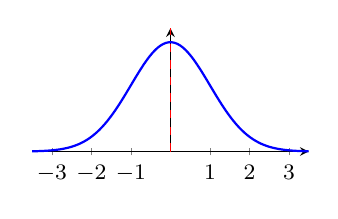
\begin{tikzpicture}[
            declare function={
                normal(\x,\m,\s) = 1 / (\s * sqrt(2 * pi)) * exp(-(\x - \m)^2 / (2 * \s^2));
                asinh(\x) = ln(\x + sqrt((\x^2) + 1));
                basex(\x,\m,\s) = (\x - \m) / \s;
                bigh(\x,\m,\s,\e,\d) = sinh(\d * asinh(basex(\x, \m, \s)) - \e);
                smallh(\x,\m,\s,\e,\d) = \d * cosh(\d * asinh(basex(\x, \m, \s)) - \e) / (\s * sqrt(2 * pi * (1 + ((basex(\x, \m, \s))^2))));
                sinhdist(\x,\m,\s,\e,\d) = smallh(\x, \m, \s, \e, \d) * exp(- 0.5 * ((bigh(\x, \m, \s, \e, \d))^2));
            }]
            \begin{axis}[
                footnotesize,
                clip=false,
                domain=-3.5:3.5,
                samples=100,
                ytick=\empty,
                %legend entries={Sim\'etrica\\Positiva\\Negativa\\},
                legend pos=south east,
                %legend style={font=\footnotesize},
                width=0.42\textwidth,
                height=0.2595797280593325\textwidth,
                axis lines=middle,
                %grid=major,
                no markers,
                ]
                \addplot+[thick] {normal(x, 0, 1)};
                \addplot+[dashed, forget plot] coordinates {(0, 0) (0, 0.45)};
                %\node[pin=180:Media] at (axis cs:0,0.1) {};
                %\node[pin=180:Mediana] at (axis cs:0,0.2) {};
                %\node[pin=180:Moda] at (axis cs:0,0.3) {};
            \end{axis}
        \end{tikzpicture}
        &
        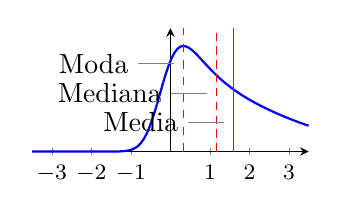
\begin{tikzpicture}[
            declare function={
                normal(\x,\m,\s) = 1 / (\s * sqrt(2 * pi)) * exp(-(\x - \m)^2 / (2 * \s^2));
                asinh(\x) = ln(\x + sqrt((\x^2) + 1));
                basex(\x,\m,\s) = (\x - \m) / \s;
                bigh(\x,\m,\s,\e,\d) = sinh(\d * asinh(basex(\x, \m, \s)) - \e);
                smallh(\x,\m,\s,\e,\d) = \d * cosh(\d * asinh(basex(\x, \m, \s)) - \e) / (\s * sqrt(2 * pi * (1 + ((basex(\x, \m, \s))^2))));
                sinhdist(\x,\m,\s,\e,\d) = smallh(\x, \m, \s, \e, \d) * exp(- 0.5 * ((bigh(\x, \m, \s, \e, \d))^2));
            }]
            \begin{axis}[
                footnotesize,
                clip=false,
                domain=-3.5:3.5,
                samples=100,
                ytick=\empty,
                %legend entries={Sim\'etrica\\Positiva\\Negativa\\},
                legend pos=south east,
                %legend style={font=\footnotesize},
                width=0.42\textwidth,
                height=0.2595797280593325\textwidth,
                axis lines=middle,
                %grid=major,
                no markers,
                ]
                %\addplot+[dashed, forget plot] coordinates {(0, 0) (0, 0.45)};
                %\addplot+[thick] {normal(x, 0, 1)};
                \addplot+[thick] {sinhdist(x, 0, 1, 1, 1)};
                \addplot+[forget plot] coordinates {(1.591846220604143, 0) (1.591846220604143, 0.42)};
                \addplot+[densely dashed, forget plot] coordinates {(1.1752, 0) (1.1752, 0.42)};
                \addplot+[dashed, forget plot] coordinates {(0.3295046, 0) (0.3295046, 0.42)};
                %\addplot+[dashed, forget plot] coordinates {(-1.591846220604143, 0) (-1.591846220604143, 0.42)};
                %\addplot+[dashdotted, forget plot] coordinates {(-1.1752, 0) (-1.1752, 0.42)};
                %\addplot+[densely dashed, forget plot] coordinates {(-0.3295046, 0) (-0.3295046, 0.42)};
                %\addplot+[thick] {sinhdist(x, 0, 1, -1, 1)};
                %\node[pin=180:Media] at (axis cs:1.591846220604143,{sinhdist(1.591846220604143, 0, 1, 1, 1)}) {};
                \node[pin=180:Media] at (axis cs:1.591846220604143,0.1) {};
                %\node[pin=180:Mediana] at (axis cs:1.1752,{sinhdist(1.1752, 0, 1, 1, 1)}) {};
                \node[pin=180:Mediana] at (axis cs:1.1752,0.2) {};
                %\node[pin=180:Moda] at (axis cs:0.3295046,{sinhdist(0.3295046, 0, 1, 1, 1)}) {};
                \node[pin=180:Moda] at (axis cs:0.3295046,0.3) {};
                %\node[pin=180:Media] at (axis cs:-1.591846220604143,{sinhdist(1.591846220604143, 0, 1, 1, 1)}) {};
                %\node[pin=180:Mediana] at (axis cs:-1.1752,{sinhdist(1.1752, 0, 1, 1, 1)}) {};
                %\node[pin=180:Moda] at (axis cs:-0.3295046,{sinhdist(0.3295046, 0, 1, 1, 1)}) {};
            \end{axis}
        \end{tikzpicture}
        \\
        Negativa & Simétrica & Positiva \\
    \end{tabular}
        %\includegraphics[width=0.34\textwidth]{exponente_momentos}
    \end{center}
    \begin{block}{Recordar}
        \begin{itemize}
            \item Coeficiente de variación (inversa de razón señal ruido): $\frac{s}{\bar{x}} = \sqrt{\frac{\bar{m}_{2}}{\bar{x}^{2}}}$.
        \end{itemize}
    \end{block}
\end{frame}

\begin{frame}
    \frametitle{Cuarto momento: curtosis / apuntamiento (\emph{kurtosis})}
    \begin{block}{Coeficiente}
        \begin{equation*}
            \frac{\bar{m}_{4}}{s^{4}} - 3 .
        \end{equation*}
    \end{block}
    \begin{center}
        %\includegraphics[width=0.5\textwidth]{kurtosis}
        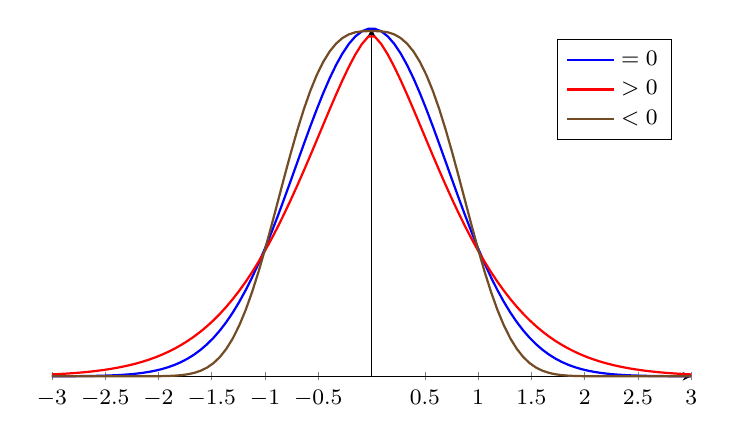
\begin{tikzpicture}
            \begin{axis}[
                footnotesize,
                clip=false,
                domain=-3:3,
                samples=100,
                ytick=\empty,
                legend entries={$= 0$\\$> 0$\\$< 0$\\},
                legend pos=north east,
                %legend style={font=\footnotesize},
                width=0.8\textwidth,
                height=0.49443757725587145\textwidth,
                axis lines=middle,
                %grid=major,
                no markers,
                ]
                \addplot+[thick] {exp(-x * x) / 1.77245385091};
                \addplot+[thick] {exp(-pow(abs(x), 1.5)) / 1.805490586};
                %\addplot+[thick] {exp(-pow(abs(x), 1.25)) / 1.862767542};
                %\addplot+[thick] {exp(-pow(abs(x), 5)) / 1.8363374848};
                \addplot+[thick] {exp(-pow(abs(x), 3)) / 1.7859590231};
                %\addplot+[thick] {exp(-x * x * x * x) / 1.812804954};
            \end{axis}
        \end{tikzpicture}
    \end{center}
    \begin{alertblock}{}
        \begin{itemize}
            \item ¿3?
        \end{itemize}
    \end{alertblock}
\end{frame}

\begin{frame}
    \frametitle{Medidas de concentración}
    \begin{block}{Curva de Lorenz}
        \begin{equation*}
            u_{i} = \frac{i}{n} ,
        \end{equation*}
        \begin{equation*}
            v_{i} = \frac{\sum_{p = 1}^{i} x_{\parens{p}}}{\sum_{p = 1}^{n} x_{\parens{p}}} .
        \end{equation*}
    \end{block}
    \begin{center}
        \includegraphics[width=0.9\textwidth]{lorenz}
    \end{center}
\end{frame}

\begin{frame}
    \frametitle{Medidas de concentración}
    \begin{block}{Coeficiente de Gini}
        \begin{itemize}
            \item $G = 2 F$.
            \item $F = \sum_{i = 1}^{n} F_{i} - \frac{1}{2}$, con $F_{i} = \frac{\parens{u_{i - 1} + u_{i}} \parens{v_{i} - v_{i - 1}}}{2}$.
            \item $G = 1 - \frac{1}{n} \sum_{i = 1}^{n} \parens{v_{i - 1} + v_{i}}$.
        \end{itemize}
    \end{block}
    \begin{center}
        \includegraphics[width=0.4\textwidth]{gini}
        \includegraphics[width=0.45\textwidth]{gini_ejemplo}
    \end{center}
\end{frame}

\iffalse
\begin{frame}[allowframebreaks, noframenumbering]
\frametitle<presentation>{References}
\printbibliography
%\bibliographystyle{apalike}
\end{frame}
\fi



\end{document}
